\chapter{OpenFOAM}

OpenFOAM ist ein in C++ geschriebenes Framework zum lösen von partiellen Differentialgleichungen. Hauptanwendungsbereich ist die numerische Strömungssimulation, aber auch Finanzmathematik und mechanische Analysen sind möglich. 

\section{Installation}

Grundsätzlich stehen zwei verschiedene Installationswege zur Verfügung: Das Übersetzen des Quellcodes in Maschinencode (als Kompilation bezeichnet) oder die Installation mit Hilfe eines Paketmanagers.

\todo{installationsanweisungen}

\section{Struktur}

Zur Simulation einer Problemstellung wird zunächst ein eigenes Verzeichnis mit beliebigem Namen benötigt.
Die Struktur innerhalb dieses ist jedoch fest vorgegeben. \autoref{fig:struktur} zeigt die Struktur innerhalb des Simulationsordners.

\begin{figure}
\centering
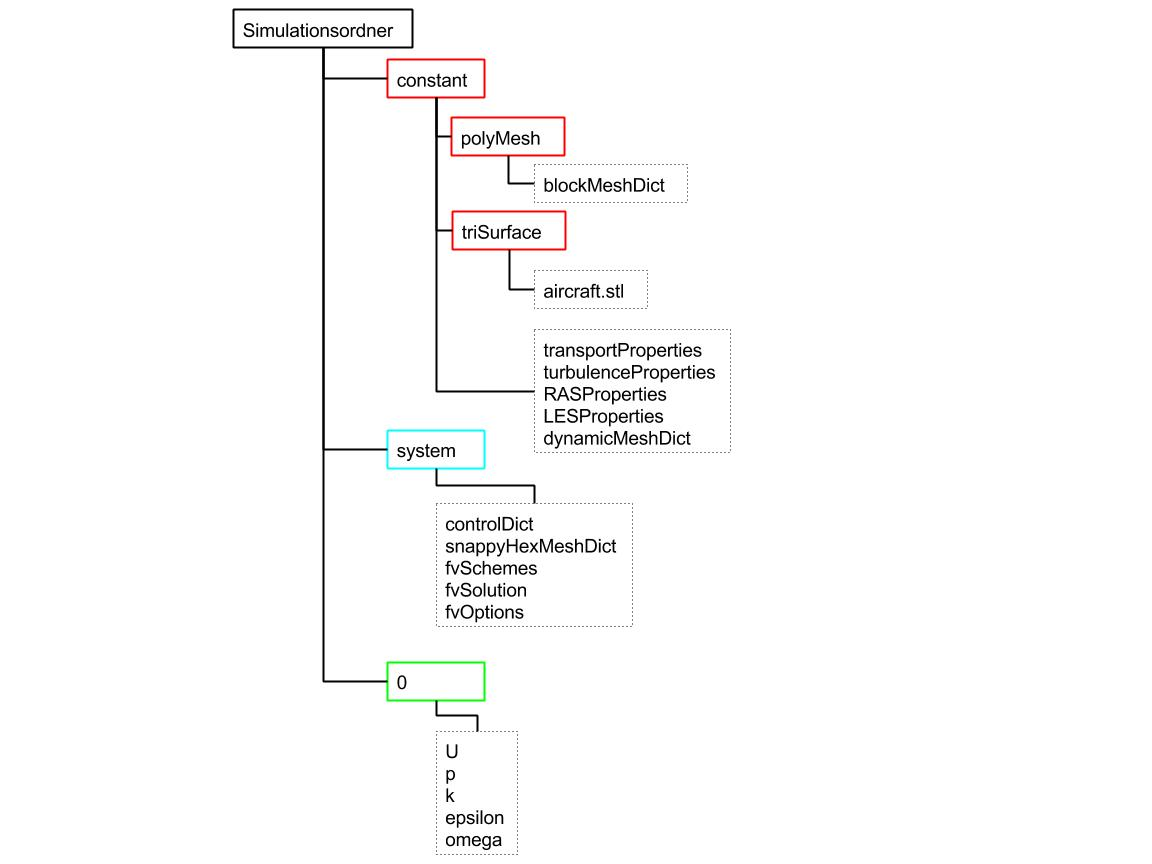
\includegraphics[width=\linewidth]{Abbildungen/Struktur}
\caption[Struktur einer OpenFOAM Simulation]{Die Ordnerstruktur innerhalb einer OpenFOAM Simulation. Der system ordner beinhaltet die Einstellungen der Lösungsprogramme, der 0 Ordner beinhaltet die Initialbedingungen und der constant Ordner das Gitter und die Randbedingungen}
\label{fig:struktur}
\end{figure}

\subsection{\texttt{constant}}
Der \textit{constant} Ordner beinhaltet im Subordner polyMesh das von numerische Gitter im OpenFOAM Format. Handelt es sich bei dem Gitter um ein mit \textit{blockMesh} generiertes blockstrukturiertes Gitter, so liegt dort auch die Datei \textit{blockMeshDict}, Siehe \autoref{lst:blockMeshDict}, innerhalb derer die Geometrie und die Randbedingungen definiert werden. Des Weiteren beinhaltet \textit{constant} unter Umständen das Unterverzeichnis \textit{triSurface}, innerhalb dessen Oberflächengitter zur Generierung komplexer Gitter mit den Gittergeneratoren \textit{snappyHexMesh}, \textit{foamyQuadMesh} und \textit{foamyHexMesh} abgelegt sind (Siehe Kapitel Gittergenerierung).

Zwangsweise vorhanden sein muss die Datei transportProperties. Diese Datei legt die kinematische Viskosität sowie die Art von Fluid (Newtonsch, Binghamsch, etc.) fest.

In den Dateien RASProperties, LESProperties und turbulenceProperties werden etwaige Turbulenzemodelle definiert. 

Eine gesonderte Rolle spielte die Datei dynamicMeshDict; Soll innerhalb der Simulation mit bewegten Gittern gearbeitet werden, so wird das Verfahren, sowie die Bewegung hier definiert.

\subsection{\texttt{system}}
Mit den Dateien innerhalb dieses Ordners wird die Simulation gesteuert.

\begin{itemize}
	
	\item[\textbf{\textit{controlDict}}] Mit dieser Datei wird die Simulation gesteuert; nachfolgend sind die wichtigsten Parameter und ihre Optionen aufgeführt.
		\subitem application : legt den zu verwendenden Gleichungslöser fest; nicht zwingend notwending, nur in Kombination mit den von OpenFOAM bereitgestellten RunFunctions benötigt.
		
		\subitem startFrom : legt fest ob die Simulation von einem festgelegten Zeitpunkt aus startet oder vom letzten verfügbaren Zeitschritt. Soll ein Zeitschritt festgelegt werden, muss als Wert 'startTime' eingetragen werden. Ansonsten 'latestTime'. 
		
		\subitem startTime : wird nur benötigt falls ein fester Startzeitpunkt festgelegt werden soll. 
		
		\subitem endTime : definiert das Ende der Simulation. 
		
		\subitem deltaT : bezeichnet die Zeitschrittweite und bei instationären Simulationen damit die Courantzahl. Bei stationären Zeitschritten ist die Zeitschrittweite überflüssig, auf 1 gesetzt zeigt sie somit die Anzahl an Iterationen an. 
		
		\subitem writeControl : steuert das Speichern. Soll der momentan gerechnete Zeitschritt noch beendet werden und danach die Simulation abgeschlossen, muss als Wert 'writeNow' eingetragen werden. Andere Optionen sind timeStep und XXX \todo{anderen Parameter raussuchen}.
		
		\subitem writeInterval : definiert die Speicherintervalle.
		
		\subitem writeFormat : definiert ob beim speichern die Daten in binärem Format oder in menschlich-lesbarem (ascii) gespeichert werden sollen. Binary reduziert den benötigten Speicherplatz auf etwa 20 \% des menschlich-lesbaren.
		
		\subitem runTimeModifiable : lässt zu ob Textdateien zur Kontrolle der Simulation geändert und damit die Simulation zur Laufzeit modifiziert werden darf.
		
		\subitem functions : Soll zur Laufzeit bereits PostProcessing betrieben werden (bspw: grafische Schnitte, Strömungsbeiwerte, etc), müssen diese hier definiert werden
	
	\item[\textbf{\textit{snappyHexMeshDict}}] Diese Datei wird als Steuerdatei für den Gittergenerator \textit{snappyHexMesh} benötigt. Details dazu finden sich im Kapitel Gittergenerierung.
		
	\item[\textbf{\textit{fvSchemes}}] Diese Datei beinhaltet die zu verwendenden Diskretisierungs und Interpolationsverfahren. Grundsätzlich gibt es in OpenFOAM viele verschiedene Verfahren. Erforderlich für das Starten einer Simulation ist zunächst, dass alle in den vorhandenen Gleichungen auftretenden Terme durch die Verfahren abgedeckt sind. \autoref{tab:terme} zeigt die Terme und ihre Bezeichnungen in OpenFOAM. Das Kapitel Diskretisierungen behandelt die vorhandenen Verfahren und ihre Effekte.
	
	\begin{table}[htb]
	  \centering
	  \begin{tabular}{m{6cm}m{3cm}} 
	  \toprule
	    	Term & Bezeichnung in OpenFOAM \\
	  \midrule
			Instationärer Term $ \frac{\partial u_{i}}{\partial t} $ & \texttt{ddtSchemes} \\
			Konvektiver Term $ u_{j} \frac{u_{i}}{x_{j}} $ & \texttt{divSchemes} \\
			(Druck)Gradient $ - \frac{ \frac{p}{\rho} + g k}{\partial x_{i}} $ & \texttt{gradSchemes} \\
			Diffusiver Term $ \nu \frac{\partial^{2} u_{i}}{\partial u_{j}^{2}} $& \texttt{laplacianSchemes} \\
			Interpolationsverfahren & \texttt{interpolationSchemes} \\
	  \bottomrule
	  
	  \end{tabular}
	  \caption[Terme und ihre Bezeichnungen in OpenFOAM]{Terme und ihre Bezeichnungen in OpenFOAM}
	  \label{tab:terme}
	\end{table} 
	
	\item[\textbf{\textit{fvSolution}}] Innerhalb dieser Datei werden die Algorithmen zur Gleichungslösung eingestellt. Des Weiteren werden Ralaxationsfaktoren und Konvergenzkriterien hier definiert. 
	
	\item[\textbf{\textit{fvOptions}}] Diese Datei beinhaltet die Beschreibung bestimmter Patches, beispielsweise zur Simulation von porösen Medien oder zur Simulation mit anderen Bezugssystemen. 
	
\end{itemize}

\subsection{\texttt{0}}
Innerhalb des '0' Ordners werden die Initialbedingungen festegelegt; alle zur Simulation benötigten Größen erhalten ihre eigene Datei, innerhalb derer die Initialwerte festgelegt werden. Für Details: Kapitel Initial und Randbedingungen. 




\newpage